\chapter{Foundations}
\label{chp:foundations}

This chapter provides information on overarching as well as foundational concepts relevant to the following chapters. Specifically, we cover two areas.

\begin{enumerate}
    \item \textbf{Scholarly Data}\\
        First, we give an overview of the academic publication ecosystem and its relation to the landscape of scholarly data. Understanding the parts involved and relations between them is helpful for understanding decisions made in the system design and method development of the approaches presented later on. Based on the overview, we additionally highlight the current state-of-the-art.
    \item \textbf{Data Mining \& Information Extraction}\\
        Second, we present essential concepts from the areas of data mining and information extraction. These are needed for the quantification of the research goals as well as the results that are presented later on.
\end{enumerate}

Explanations of concepts that are specific to the work presented in individual chapters, as well as a focussed view on state-of-the-art approaches in the respective areas, are provided jointly with the approaches in Chapters \ref{chp:corpus}\,--\,\ref{chp:params}.

\section{Scholarly Data}

% What do I want to say and convey here?

% - what's the general nature of scholarly data?
%   -> structured representation of publication [meta]data that is the basis for (1) digital services in academia, (2) analyses, (3) ML model dev+evaluation

%                 (TODO)
% TODO: define ``scholarly data'' more clearly
%       - what's special about it?
%       - difference to e.g. patents, news, etc.?
%                 (TODO)

The term ``scholarly data'' is used to refer to data that represents academic publications or related concepts, such as authors and their affiliations. It can coarsely be divided into data directly reflecting the \emph{content} of publications, and metadata, which gives information \emph{about} publications.
As such, scholarly data is the basis for essentially everything that relies on digital processing of publications. The following are three key examples.
\begin{enumerate}
    \item \textbf{Digital services} in academia such as search (e.g. Google Scholar\refurl{https://scholar.google.com/}{2023-11-06}, Semantic Scholar\refurl{https://www.semanticscholar.org/}{2023-11-06}), recommendation (e.g. Academia.edu\refurl{https://www.academia.edu/}{2023-11-06}, CORE Recommender\refurl{https://core.ac.uk/services/recommender}{2023-11-06}), and aggregation platforms (e.g. Papers With Code\refurl{https://paperswithcode.com/}{2023-11-06}, Scopus\refurl{https://www.scopus.com/}{2023-11-06}).  % TODO: consider adding whats bad if data incorrect
    \item \textbf{Analyses} such as bibliometric analyses across time, geographic regions, or institutions, as well as trend analyses and investigations into specific phenomena like citation inequity.
    \item \textbf{Model development} such as the training and evaluation of transformer based large language models (LLMs) as well as task specific models (e.g. for recommender systems, impact prediction, or information extraction).
\end{enumerate}

Because scholarly data is only a secondary product to the actual publications themselves, it is necessary to consider how the data comes into being.

\subsection{Origins of Scholarly Data}

% - how is scholarly data generated
%   -> to some degree manually (metadata provided by authors), everything else (structured representations of full-text, references, etc.) out of necessity automated
% - what are the data sources and their peculiarities?
%   -> (see fig 2.1; from 3 stages of publishing, overall visual first, some special treatment for some metadata (wrt. access and requiring authors to manually provide it)

\begin{figure}[bt]
  \centering
  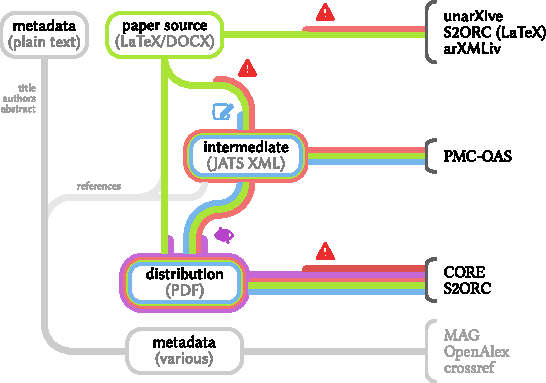
\includegraphics[width=\linewidth]{figures/foundations/scholarly_data_lifecycle}
  \caption[Schematic depiction of the origins of scholarly data]{Schematic depiction of the origins of scholarly data. Symbols indicate (1) {\color{warningsign-red}\faWarning} error-prone automated processing to extract structural and semantic information, (2) {\color{manualcheck-blue}\faPencilSquareO} a manual check, and (3) {\color{visualformat-purple}\faLowVision} loss of structural information due to transformation into a visual format. Note that physical paper sources which require OCR of scans for the creation of scholarly data are not depicted.}
  \label{fig:foundations-datalifecycle}
\end{figure}

Figure~\ref{fig:foundations-datalifecycle} schematically shows the path of a publication from authorship to distribution, together with different stages from which scholarly data can emerge. It is essential to note that academic publications are, historically and at the time of writing still, primarily written by humans with human readership in mind. As such, publications are primarily a visual medium, optimized for parsing by human vision and intelligence. Scholarly data, however, is intended for automated processing and therefore benefits, for example, from strict syntactic rules and no reliance on assumed background knowledge. As a consequence, the creation of scholarly data requires bridging between the existing visual presentation and desired structural derivate.

Specifically, this means that information which is not made explicit in publications needs to be retroactively added. For example, whether a piece of text \textit{``[1,3]''} in a publication is expressing an interval of real numbers, or a citation for references 1 and 3. Because it would be impractical to require researchers to produce a detailed set of annotations in addition to all their publications,\footnote{This can be seen as a case of the ``authoring problem'' challenging the semantic web community~\cite{Kohlhase2010}.}\textsuperscript{,}\footnote{An exception to this is basic metadata such as title, authors, and abstract, which are commonly requested to be filled into a form in plain text during the submission process of a manuscript.} the retroactive adding of information needs to be done automatically, i.e. by means of information extraction. An shown in Figure~\ref{fig:foundations-datalifecycle}, the information extraction can happen at any given stage of publication. At each stage, the nature of the available data and information is different. Accordingly, there are different benefits and challenges in each case. In the following, we will discuss these different types of data from an information extraction perspective, beginning with \LaTeX\ as it is the most relevant to the presented work.

\subsubsection{Types of Data Sources}

Viable input formats for the creation of scholarly data differ in terms of the contained information, challenges for information extraction, availability, and use.
These are discussed in the following, with Table~\ref{tab:document_formats} providing an overview.

\begin{table}[tb]
  \caption{Comparison of Scholarly Data Sources}
  \label{tab:document_formats}
  \centering
  \begin{small}
    \begin{threeparttable}
      \begin{tabular}{lcclc}
        \toprule
        Source & Doc Structure & Semantic & Open Availability & Disciplines \\
        \midrule
        LaTeX  & \checkmark    & partial\tnote{a}  & \checkmark~(arXiv)  & physics, math, CS \\
        Word   & \checkmark    & partial\tnote{b}  & $\times$~(publisher internal & all\tnote{c} \\
        JATS   & \checkmark    & \checkmark & \checkmark~(PMC OAS)   & biomedical \\
        PDF    & $\times$      & $\times$   & \checkmark~(abundant)  & all  \\
        \bottomrule
      \end{tabular}
      \begin{tablenotes}
        \item[a] Semantic to some degree by use of named macros (e.g. \texttt{\textbackslash title\{\}} or \texttt{\textbackslash section\{\}}), but usage not enforced by format.
        \item[b] Semantic to the extent that the DOCX (Office Open XML) schema describes the document structure, but dependent on authors' usage of respective Word features.
        \item[c] Primarily humanities and not so much STEM fields.
      \end{tablenotes}
    \end{threeparttable}
  \end{small}
\end{table}

% - LaTeX; what is it, why is it not the end-all-be-all, and what endeavours have been there so far and are on the horizon of LaTeX development wrt. more structure and semantic information?
%   -> brief history, used primarily in STEM fields, Turing complete, document classes and packages provide semantic macros that translate in to visual representation but authors can always chose to directly describe visual presentation rather than semantic meaning, some endeavours to allow for more semantics (scholarly data specific and from accessibility POV)

\paragraph{\LaTeX}
is described as \textit{``a system for typesetting documents''}~\cite{Lamport1994}, or a \textit{``widely used language for describing the logical structure of [...] documents''}~\cite{Mittelbach2023}. At its core, \LaTeX\ provides functionalities to control the visual presentation of a document. These functionalities are combined by macros, which offer authors the means to structurally and semantically describe a document (e.g. \texttt{\textbackslash title\{\}} or \texttt{\textbackslash section\{\}}). This structural and semantic information---which gets lost when the \LaTeX\ source is compiled to PDF---
% TODO: try to find an example of a common case where authors visually denote something instead of making it explicit by a fitting macro, where the result in the PDF is indistinguishable (also factoring in hyperref which makes footnote marks, references, citations, etc. clickable)
%\texttt{\textbackslash footnote\{Example\}}\footnote{Example} an author could use \texttt{\textbackslash textsuperscript\{\thefootnote\}} creates a footnote mark\textsuperscript{\thefootnote} that, in PDF output, is visually indistinguishable from what is produced by \texttt{\textbackslash} 
%\footnote{The translation of structural components into a visual presentation is dictated by the document classes and packages providing the macros. For example, a paper author placing text between \texttt{\textbackslash begin\{abstract\}} and \texttt{\textbackslash end\{abstract\}}, will find their abstract text prefaced with ``\textbf{Abstract.}'' and set with a reduced line width when using the document class \texttt{llncs}, whereas there will be no preface and an unchanged line width when using \texttt{acmart}.}
is immensely beneficial for information extraction.
However, \LaTeX\ documents are usually a mixture structural and presentation description, which introduces challenges~\cite{Stamerjohanns2008}.
While there have been efforts to establish \LaTeX\ extensions for more rigorous semantic annotation in the document source~\cite{Krieg2004,Groza2007,Bless2023}, these have not been widely adapted so far.
There are, however, efforts by The \LaTeX\ Project\refurl{https://www.latex-project.org/}{2023-11-08} itself to support semantic annotation natively in the future~\cite{Mittelbach2020,Mittelbach2023}.

Regarding at the availability of \LaTeX\ sources, arXiv.org\refurl{https://arxiv.org/}{2023-11-08} provides open access to over 2 million papers uploaded by their authors. With its origin in physics in the 1990s~\cite{Feder2021,Ginsparg2011a}, gradual adoption in mathematics in the early 2000s, and rapid growth in computer science since the 2010s~\cite{Saier2023unarXive}, it now covers significant portions of the scientific literature in aforementioned three disciplines. Given the benefits for information extraction, \LaTeX\ sources from arXiv have been used for generating scholarly data on a small scale since at least 1998~\cite{Nanba1998}. Large-scale efforts started with a focus on mathematics in 2008~\cite{Stamerjohanns2008}. Complete conversions of the papers on arXiv.org into a scholarly data corpus including a citation network are comparatively new development with the unarXive corpus~\cite{Saier2020} presented in this dissertation, as well as S2ORC~\cite{Lo2020}.
% Joanne Cohn sending around e-prints~\cite{Feder2021,Turner2012}
% June 1991 meets Paul Ginsparg who then goes on to start arXiv~\cite{Ginsparg2011a,Ginsparg2011}

% metadata dump since 2020(?) available on Kaggle~\cite{arxiv_kaggle_dataset}

% - What about other formats?
%   -> JATS is mighty, Word is XML, triple formats are used for metadata

\paragraph{Word}
documents (DOCX files\refurl{https://www.loc.gov/preservation/digital/formats/fdd/fdd000397.shtml}{2023-11-08}) are the second major data format commonly accepted by publishers for submitting manuscripts~\cite{Johnson2018stm}. Contrary to the \LaTeX\ approach of compilation from source files, documents are edited in an interactive ``What you see is what you get'' (WYSIWYG) editor.\refurl{https://www.microsoft.com/microsoft-365/word}{2023-11-08} While DOCX files are essentially ZIP compressed XML files and contain more explicit information then PDF derivates, there are no open repositories similar to arXiv.org that provide large quantities of paper's Word source files.  % open question: do publishers keep them?

\paragraph{Journal Article Tag Suite}
(JATS) is a standardized markup format for scientific publications based on XML~\cite{Huh2014}. As depicted in Figure~\ref{fig:foundations-datalifecycle}, JATS files are not directly created by researchers, but are rather an intermediate format used by publishers, from which they derive different presentation formats of publications, such as PDF and HTML. While JATS files provide semantically richer information than \LaTeX\ or Word source files, their generation can only partially be automated and requires human oversight. Regarding availability, the PubMed Central Open Access Subset\refurl{https://www.ncbi.nlm.nih.gov/pmc/tools/openftlist/}{2023-11-06} (PMC OAS) provides over 3 million publications from the biomedical and life sciences domain in JATS XML format. While the JATS files of the PMC OAS have been used to generate a corpus of linked publications in the past~\cite{Gipp2015}, more up-to-date and widely used corpora have only used the PDF versions of the contained documents~\cite{Lo2020}.

\paragraph{PDF}
% TODO: find source of PDF being the most used medium for paper distribution and consumption
% (couldn't find explicit source in The STM Report)
is the most common distribution format for academic publications~\cite{Johnson2018stm} and accordingly, the largest open document collections are PDF files, such as CORE~\cite{core} with over 100 million documents. The PDF format does provide optional functionalities to describe the logical structure of documents in addition to the visual presentation~\cite{ISO32000-2}. However, such annotation is not an established practice in academic publishing and, accordingly, information extraction methods have to resort to heuristic approaches based on the visually presented information only~\cite{Lopez2009,Nasar2018,Faerber202x}. This makes PDF a more error-prone source than aforementioned source formats~\cite{Bast2017}.

% \paragraph{Triple Formats}  % NOTE: note a ``source format'' from which scholarly data sets are created
% RDF, Turtle, JSON-LD, ... (relevant for metadata)

\subsubsection{Types of Scholarly Data}

Conceptually, scholarly data can be divided two overarching categories: \emph{metadata} and \emph{document collections}~\cite{Nasar2018}. As a third category, we consider \emph{linked document collections}, which combine features of aforementioned two.
We briefly introduce each of the three and provide an overview in Table~\ref{tab:data_types}.

\begin{table}[tb]
  \caption{Overview of Scholarly Data Types}
  \label{tab:data_types}
  \centering
  \begin{small}
    \begin{threeparttable}
      \begin{tabular}{lclc}
        \toprule
        Type                       & Contents                             & Size\tnote{a} & Examples \\
        \midrule
        Metadata                   & Title, author, citations, etc.       & \(10^8\)              & OpenAlex, ORKG \\
        Document Collections       & Full-text                            & \(10^8\)              & CORE, arXMLiv \\
        Linked Doc. Collections    & Full-text + citation network         & \(10^7\)              & unarXive, S2ORC \\
        \bottomrule
      \end{tabular}
      \begin{tablenotes}
        \item[a] Order of publications covered by largest representatives of each type
      \end{tablenotes}
    \end{threeparttable}
  \end{small}
\end{table}

% What do I want to say and convey here?
% - what ``conceptual'' types of scholarly data are there?
%   -> metadata, document collections, linked document collections (combining former two b/c metadata usually also means citations)
% - what are current/established (``SOTA'') approaches/endeavors/projects
%   -> ORKG (very semantic but not scalable yet), arXMLiv (math focus), S2ORC (PDF source), OpenAlex (very large, ...)

\paragraph{Metadata}
provides information \emph{about} publications, rather than reflecting their full-text content. The data partially originates in already structured form provided by authors, as it is queried by publishers during manuscript submission. This includes the title, authors, as well as the abstract. Different regarding the data's origin are bibliographic references, which are also often included in metadata sets. Here, it is necessary to extract the reference information from the document submitted by an author (e.g. \LaTeX\ or Word sources). Regarding accessibility, title and author information is generally shared freely. Abstracts and references may also be openly acceptable, but this is not always the case, as evidenced by the existence of the Initiative for Open Abstracts\refurl{https://i4oa.org/}{2023-11-09} and the Initiative for Open Citations.\refurl{https://i4oc.org/}


Two examples of scholarly metadata sets are the following. (1)~OpenAlex~\cite{openalex} contains data on over 200\,M publications, their authors, affiliations, citation links, etc. Its data sources include PubMed, arXiv, academic publishers, and various institutional repositories.%\refurl{https://api.openalex.org/sources}{2023-11-09} 
 (2)~The Open Research Knowledge Graph (ORKG)~\cite{orkg1,orkg2} provides information on over 28\,k\footnote{28.020 entities of type \texttt{http://orkg.org/orkg/class/Paper} as of 2023-11-09. Determined via the ORKG SPARQL endpoint at \url{https://www.orkg.org/sparql}.} publications, their contributions, research problems addressed etc. For its data, the ORKG is largely reliant on manual or semi-automated data entry.

\paragraph{Document Collections} provide access to publications' full-text content. Because of this, they are reliant on open access publications as a data source. Furthermore, the documents either need to be licensed in a way that allows (re-)distribution, or access to the collection itself needs to be restricted accordingly. Because there are documents sources in different formats (see Figure~\ref{fig:foundations-datalifecycle}), document collections derived from them take different forms. While some are primarily aggregates of openly accessible PDFs (and therefore can also be seen as a data source), such as CORE~\cite{core}, others are the result of an involved generation process. An example for the latter is arXMLiv~\cite{arXMLiv}, which is an XML conversion of the papers on arXiv, comprising 1.6 M documents in its most recent version.

In order to use a document collection for applications involving citation information, the it has to be jointly used with a suitable set of citation metadata. This requires (1)~the citation metadata to cover the documents within the collection, and (2)~the availability of identifiers (such as DOIs) or some matching procedure.  % NOTE: could also mention that citations information is then limited to that among the documents in the collection. *not* covered are all citations where the collection documents are the citing paper --- b/c citation relations aren't that ``self contained''

\paragraph{Linked Document Collections}
are document collections that, in addition to the document contents, include a citation network. This means, that in addition to the requirements for creating a document collection, their generation involves the additional step of linking the references in the documents' reference sections. Commonly, this furthermore involves linking in-text citations to their respective references, to provide for more fine-grained citation information.

Representatives of linked document collections are CiteSeerX~\cite{Wu2015,Wu2016,Patel2021},  % Wu2015: original publication, Wu2016: data sources & pipeline details, Patel2021: most recent size number (10+ M)
S2ORC~\cite{Lo2020}, and unarXive~\cite{Saier2020}. unarXive is generated from the \LaTeX\ sources on arXiv, comprising 2\,M documents in its most recent version. Being generated from arXiv, it covers physics, mathematics, and computer science publications. CiteSeerX and S2ORC are both generated from PDF files of various sources, such as PubMed and publishers' websites, and contain over 10\,M and 12\,M documents respectively. The publications covered are from various fields including medicine and biology, physics, mathematics, and computer science.

% \subsection{State-of-the-Art}
% TODO: put SOTA here? would need to compare by some criteria, which should be introduced in data quality section below ... so, as third section in foundations chapter mby?

\section{Data Mining \& Information Extraction}

% What do I want to say and convey here? (TODO: integrate in text)
% - Data Quality: defining goal and assessment of results wrt. scholarly data produced
% - Model Evaluation: assessment of extraction models

% ``Data Mining is the process of discovering useful patterns and trends in large data sets.''~\cite{Larose2014}
% Information Extraction the process of ``converting unstructured text into a structured representation''~\cite{Aggarwal2018}

The work presented in this dissertation aims to improve the quality of scholarly data, and involves both data mining, the process of ``discovering useful patterns and trends in large data sets''~\cite{Larose2014}, and information extraction, the process of ``converting unstructured text into a structured representation''~\cite{Aggarwal2018}. In the following, we therefore provide background information regarding (1)~data quality, and (2)~the evaluation of information extraction models. Based on the considerations and concepts introduced, the goals and results of the work presented in the following chapters can be quantitatively assessed.

\subsection{Data Quality}\label{sec:foundations-dataquality}

% Side note: could mention that bibliometrics/scientometrics/science of science is also concerned w/ other aspects not covered below, but these are not ``(big) data driven''

Data quality is commonly understood as being context specific. In a very general, quantitative way, data quality is accordingly defined as ``fitness for use''~\cite{Strong1997,Juran1999}. Meaningful metrics for data quality in the context of scholarly data can therefore be derived by considering its use. Because existing literature on scholarly data quality only considers specific use cases and offers no systematic consideration of the topic~\cite{Strotmann2015,Lauscher2018}, we present a structured, more encompassing perspective in the following.

\subsubsection{Data Quality in the Context of Scholarly Data}

Historically, the dominant use of scholarly data is found in bibliometric and scientometric analyses~\cite{Garfield1964,Mingers2015}, such as impact or performance analysis and trend detection. The focus of use in that case lies on the citation network. % NOTE: also involves the aspect of author disambiguation
More recently, with the continuing rise of open access publishing and advances in NLP, additional areas of significant use have been established. These are training ML models~\cite{Gudivada2017}, and analyses of publications' full-text content~\cite{Jurgens2018,Lahav2022}. While the citation network remains a key focus area for scholarly data use~\cite{Wu2022doceng}, these recent usage patterns additionally put importance on structured representations of the publication content.

Key dimensions of data quality most commonly cited in the literature are (1)~relevance, (2)~accuracy, (3)~timeliness, (4)~comparability, and (5)~completeness~\cite{Herzog2007}. Based on these general dimensions and aforementioned focus areas of scholarly data use, quality criteria for scholarly data can be derived, as shown in Table~\ref{tab:scholdataquali}. In the following, we discuss the five dimensions with regard to scholarly data, as well as the quality criteria derived based on the focus areas of use.

\begin{table}[tb]
  \caption{Scholarly Data Quality Criteria}
  \label{tab:scholdataquali}
  \centering
  \begin{small}
    \begin{threeparttable}
      \begin{tabular}{lll}  % p{9.7cm}
        \toprule
        Dimension & Focus\tnote{a} & Specific Criterion\\
        \midrule
        \multirow{2}{*}{Relevance} & CN & \textbf{C1} Representative coverage of publications in target area \\
        \ & SDR & \textbf{C2} Inclusion of relevant content types (text, formulae, tables, etc.) \\
        \arrayrulecolor{lightgrey}\hline\arrayrulecolor{black}
        \multirow{2}{*}{Accuracy} & CN & \textbf{C3} Correctly linked references \\
        \ & SDR & \textbf{C4} Noise-free full-text content \\
        \arrayrulecolor{lightgrey}\hline\arrayrulecolor{black}
        \multirow{2}{*}{Timeliness} & \multirow{2}{*}{(both\tnote{b}~\,)} & \multirow{2}{*}{\textbf{C5} Coverage of recent publications} \\
        \ & \ & \ \\
        \arrayrulecolor{lightgrey}\hline\arrayrulecolor{black}
        \multirow{2}{*}{Comparability} & CN & \textbf{C6} Use of established document identifiers (DOI, PubMed ID, etc.) \\
        \ & SDR & \textbf{C7} Fine-granular, specifically typed content representation \\
        \arrayrulecolor{lightgrey}\hline\arrayrulecolor{black}
        \multirow{2}{*}{Completeness} & CN & \textbf{C8} All references of included publications successfully linked \\
        \ & SDR & \textbf{C9} No sections or content missing (appendices, formulae, etc.) \\
        \bottomrule
      \end{tabular}
      \begin{tablenotes}
        \item[a] Focus are of use (CN = Citation Network, SDR = Structured Document Representation)
        \item[b] Bundled together because the timeliness of a publication's content (SDR focus), is bound to the timeliness of the of publication itself (CN focus). In other words, parts of the document don't change independently after publication.
      \end{tablenotes}
    \end{threeparttable}
  \end{small}
\end{table}

\begin{enumerate}
    \item \textbf{Relevance} is a quality dimension heavily dependent on the data's intended use. As scholarly data is used to gain insight on particular aspects of academia (e.g. a certain field, practice, institution or individual), the data needs to cover that aspect to a sufficient degree in order to be relevant. For citation based analyses, this means a representative portion of publications from the studied disciplines, time span, languages, etc. has to be covered. On the level of document representations, it is important that relevant content types are included. For example, for a comparison of mathematical formula usage in publications, the data has to contain publications' full-text \emph{including} pieces and sections of mathematical notation.  % generalization: volume (the more publications, the more general coverage)
    \item \textbf{Accuracy} regarding the citation network means, that references should be correctly linked to the publications they are referencing. For document representations, accuracy entails that text content should be free of noise. As described in the previous sections, both of these are non-trivial due to the sources scholarly data relies on. Regarding the question of how accurate scholarly data has to be for meaningful usage, previous research proposes that for ``local analyses'' (e.g. node degrees in a citation network) 80\% correct data can already allow for reasonable insight, but for ``global analyses'' (e.g. rankings) at least 90\% correctness should be aimed for~\cite{Strotmann2015}. Others have argued that quality requirements in scientometrics are high enough to warrant the cost of requiring a ``human in the loop'' approach to data generation~\cite{Lauscher2018}.  % argument for LaTeX
    \item \textbf{Timeliness} with regard to scholarly data is crucial if the underlying reality of the research object changes quickly. In cases like training a model for parsing bibliographic references, recent data is likely not needed, as citation styles don't change rapidly.  However, for tasks like paper recommendation, everything published after the recommender model's training data simply can not be recommended. Accordingly the coverage of recent publications is desirable.  % TODO: mention that ``timely'' depends on publications as a primary object of consideration, and therefore distinguishing between CN and SDR does not make sense  % argument for continuous generation (possible w/ unarXive code, not implemented though; also: matching to target set more easily updatable than clustering)
    \item \textbf{Comparability} as a quality criterion is of importance to enable the combined use of data sets. In other words, items in the data set should be clearly identified. In the case of scholarly data, this calls for determining the persistent identifiers (e.g. DOI, ORCiD, and ROR~\cite{Meadows2019}) of items of interest. For the citation network specifically, this means providing document identifiers. Regarding a structured document representation, comparability of contents can be facilitated by providing a fine-grained, typed content representation---for example, by representing a publications' text structured into sections, subsections, etc.
    \item \textbf{Completeness} of data means that no records are missing \emph{and} records are not missing any attributes. Regarding scholarly data, there are practical boundaries to simply aiming for including everything ever published (e.g. closed access publications and distribution rights). It is reasonable, however, to strive for a complete citation network, i.e. that all entries in the reference section of a given publication are successfully linked. For a structured document representation, completeness means that no parts of the content or types of content are missing (e.g. appendices, formulae, etc.). % could also mention metadata (e.g. not missing author information)
\end{enumerate}

Based on these considerations, and the resulting quality criteria \textbf{C1\,--\,C9} presented in Table~\ref{tab:scholdataquali}, a quantitative view on the goal of the presented work (enabling higher quality scholarly data) and achieved results is possible.
% Scholarly data provided specifically for a narrowly defined use case naturally ...
For each chapter, we present a summary box as the one shown below.\footnote{Result indicator (``Res.'') \textbf{+}: SOTA/improvement/etc. (see explanation), =: equal to previous, $\circ$: not considered.}

\begin{infobox-progress}
      \textbf{Scholarly Data Quality Contributions - [Example]}\vspace{0.5em}

      \begin{tabular}{cp{11.3cm}}
        \toprule
        Crit. & Explanation \\
        %Crit.\footnote{Quality criterion (see Table~\ref{tab:scholdataquali}} & Res.\footnote{Result\\\textbf{+}: SOTA/improvement/etc. (see explanation)\\=: equal to previous\\$\circ$: not considered.} & Explanation \\
        \midrule
        \textbf{C1} & Improvement of relevance, by adding ... to the citation network. \\
        \textbf{C2} & Improvement of relevance, by adding ... to the structured document representation. \\
        ... & ... \\
        \textbf{C9} & Improvement of completeness of document representation, by .... \\
        \bottomrule
      \end{tabular}

      % \vspace{1em}
      % \begin{footnotesize}
      % \textbf{Lagend:}~~\textbf{+}: SOTA/improvement~~{\color{contextgrey}|}~~=: equal to previous~~{\color{contextgrey}|}~~$\circ$: not considered
      % \end{footnotesize}
\end{infobox-progress}

In the following section we present the tools to quantitatively assess the information extraction models that enable the improved scholarly data.

\subsection{Model Evaluation}

Model evaluation is what's guiding the development and assessment of approaches to computational problems. For example, when developing a machine learning approach to a classification problem, it is of interest to compare the approach to existing ones. In essence, a model evaluation results in a performance estimate. This is because the model performance can not be known in advance for every possible input, so only an estimate based on a set of realistic inputs can be attained.
To get a performance estimate, the model is applied on inputs, for which the desired output is already known---a \emph{ground truth}. The model outputs are then compared with the desired outputs to by means of \emph{evaluation metrics}. In the following, we describe the means of such output comparisons, as well as several evaluation metrics.

\subsubsection{Basic Concepts}

For the scope of the works presented in this dissertation, model predictions as well as ground truths can be regarded as labels. Accordingly, comparisons in an evaluation are between predicted labels and ground truth labels.

\paragraph{Confusion Matrix} The most basic elements in a comparison between predicted labels and actual (ground truth) labels can be arranged in a \emph{confusion matrix}, as shown below for a binary classification with labels Positive (Pos.) and Negative (Neg.).

\begin{center}
{    % for making group where "\makegapedcells" is valid
\makegapedcells
\begin{tabular}{cc|cc}
\multicolumn{2}{c}{}
            &   \multicolumn{2}{c}{Predicted} \\
    &       &   Pos. &   Neg.            \\
    \cline{2-4}
\multirow{2}{*}{\rotatebox[origin=c]{90}{Actual}}
    & Pos.  & TP    & FN                \\
    & Neg.  & FP    & TN                \\
    \cline{2-4}
    \end{tabular}
 }
\end{center}

% \begin{equation*}
% \begin{array}{cc|cc}
%     & \ & \multicolumn{2}{c}{\text{Ground Truth Label}} \\
%     & \ & \text{Positive} & \text{Negative} \\
%     \hline
%     \multirow{2}{*}{Predicted Label} & \text{Positive} & \text{True Positives (TP)} & \text{False Positives (FP)} \\
%      & \text{Negative} & \text{False Negatives (FN)} & \text{True Negatives (TN)} \\
% \end{array}
% \end{equation*}

Based on the True Positives (TP), False Positives (FP), False Negatives (FN) and True Negatives (TN), different metrics can be calculated.

\paragraph{Accuracy} expresses the overall ratio of correct predictions in an evaluation, calculated over both the correct positive, and the correct negative predictions.

\begin{equation*}
\text{Accuracy (ACC)} = \frac{\text{TP + TN}}{\text{TP + TN + FP + FN}}
\end{equation*}

Accuracy is informative in evaluations where the labels are balanced, but of limited information value when this is not the case. In such cases, the metrics precision and recall should be regarded.

\paragraph{Precision} expresses for the set of positive predictions, what ratio of these was made correctly.

\begin{equation*}
\text{Precision (P)} = \frac{\text{TP}}{\text{TP + FP}}
\end{equation*}

\paragraph{Recall} expresses for the set of ground truth positives, what ratio of these was correctly predicted positive.

\begin{equation*}
\text{Recall (R)} = \frac{\text{TP}}{\text{TP + FN}}
\end{equation*}

Achieving a good precision and recall with a model is always a trade-off. This can be illustrated by the fact that a model which always predicts a positive label will achieve a perfect recall of 1.\footnote{Always predicting a positive label ensures $\text{FN} = 0$, which means $\text{R} = \frac{\text{TP}}{\text{TP + FN}} = \frac{\text{TP}}{\text{TP} + 0} = \frac{\text{TP}}{\text{TP}} = 1$.} Because then all ground truth positives will be predicted correctly, but in turn all ground truth negatives will be predicted incorrectly.

\paragraph{F-score}
is a means to quantify precision and recall in a single value. Its general form, $\text{F}_\beta$, allows to put more weight on either the precision or recall. Setting $\beta$ to 1 gives the $\text{F}_1$, which is the harmonic mean of precision and recall.

\begin{equation*}
\text{$\text{F}_1$-score ($\text{F}_1$)} = \frac{2 \cdot \text{P} \cdot \text{R}}{\text{P + R}}
\end{equation*}

Precision, recall and, $\text{F}_1$-score are the typical metrics to assess and compare approaches to the information extraction tasks covered in this dissertation. In the following section, task specific considerations regarding model evaluation are discussed.

% part | task | metrics
% - unarXive20 | parsing | success rate
% - unarXive20 | matching->multiclass clf | success rate, accuracy? (mby precision)
% - blocking | matching->multiclass clf | p, r, f1
% - unarXive22 | matching | success rate
% - xling | language detection->clf | p, r, f1
% - hyperpie | ner->seq. labeling->clf| p, r, f1
% - hyperpie | re->binary clf | p, r, f1

\subsubsection{Task Specific Considerations}

Here we briefly present considerations regarding the evaluation of models for specific tasks. Detailed discussions can be found in the respective chapters.

\paragraph{Reference Linking}
is a task that aims to identify for a bibliographic reference, which publication it is referring to. The task is necessary because references in available data sources (PDF, \LaTeX, etc.) are first and foremost just ambiguous character strings, as they do not unanimously follow a single, rigorously defined format. Furthermore, identifying the referenced publication presupposes a given set of distinct publications (a ``target set'') from which to identify one. In an idealized model world, this target set encompasses everything that was ever referenced. Practically though, the target set is a finite set of publication records acquired from some data source. For the evaluation of reference linking models, this leads to the following consideration.

If a reference can not be linked to the target set, it stands to question if
\begin{itemize}
    \item (a) the reference publication \emph{is} part of the target set, but the matching model failed to identify it.
    \item (b) the reference publication \emph{is not} part of the target set, and the matching model correctly determined that none of the publications in the target set is the correct match.
\end{itemize}

As a consequence, the recall of a reference linking model (i.e. the ratio of successfully matched references) is influenced both by the model performance \emph{and} the selection of target set. The precision (i.e. the correctness ratio of matched references) can be understood as is.

\paragraph{Entity Recognition}
is the task of identifying entities mentioned in a text.\footnote{It is also referred to as ``Named Entity Recognition'' (NER). The term ``Named Entity Recognition and Classification'' (NERC) is sometimes used to distinguish it from only identifying mentions without assigning an entity type. Similarly, ``Named Entity Recognition and Disambiguation'' (NERD) means entities are furthermore disambiguated, which usually is done by linking to a knowledge graph.}
A key consideration regarding the evaluation of entity recognition models is whether to require \emph{exact matches} of entity mention spans (strict), or whether to also consider \emph{partial matches} (loose). For example, if a text mentions the ``Directory of Open Access Journals'' and a model only identifies ``Directory of Open Access'', this can be seen as either incorrect (strict) or correct (loose). Another consideration is whether a evaluation scheme requires the model, in addition to identifying entity mentions, to also determine each entity's type, which is common practice. The metrics typically used for evaluation are precision, recall, and $\text{F}_1$-score~\cite{Goyal2018}.

% TODO: adjust s.t. there are some considerations form which some consequence follows

\paragraph{Relation Extraction}
has to goal of determining the relations between entities mentioned in a text. It can be posed as a classification task on entity pairs. That is, for each possible combination of two entities $a$ and $b$ in a document, the task is to determine a relation label for $(a, b)$, where ``no relation'' is among the possibilities. A further distinction can be made by defining a ``none of the above'' (NOTA) label, which means the two entities \emph{are} in a relation, but there is not fitting label in the set of labels defined by the task~\cite{Bassignana2022}. % could also mention directed vs undirected relations -> strict vs loose evaluation
Relation extraction, as described above, is evaluated on an \emph{entity level}, while the text based on which relations get determined contains entity \emph{mentions}. To illustrate this, consider the following text.

\begin{quote}
\textit{``The Directory of Open Access Journals (DOAJ) currently indexes over 20k journals. Lars Bj{\o}rnshauge, who founded the DOAJ 20 years ago, is happy about that.''}
\end{quote}

The relation [Lars~Bj{\o}rnshauge]\,$\xrightarrow[]{\text{\texttt\tiny founded}}$[DOAJ] exists between two entities. The second sentence it the text with entity mentions \textit{``Lars~Bj{\o}rnshauge''} and \textit{``DOAJ''} can be regarded as the \emph{relation evidence}. The metrics typically used for evaluation are precision, recall, and $\text{F}_1$-score~\cite{Nasar2021}.

\subsubsection{Bibliographic Note}

A more general and extensive introduction to above and related concepts, with extensive pointers to further literature, can be found in~\cite{Aggarwal2018}.

% - reference linking
%   - can only check if predicted link is correct (TP/TP+FP = precision)
%   - can't check if no match is b/c not in target collection or really missed match (no FN/TN info)
% - NER
%   - 
% - RE
%   - class imbalance
%   - tricky eval when modeling with entities that have multiple mentions/surface forms
